\appendix
\section{Derivations}\label{app:theory}
\paragraph{Exact moments.} In two's complement the change of a word caused by any set of flipped bits is the sum of the single-bit jumps, so $X_w=\sum_{b:\,w(b)=w}\xi_b\Delta_b$ holds exactly. With independent $\xi_b\sim\mathrm{Bernoulli}(r_b)$, $\E X_w=\sum r_b\Delta_b$ and $\mathrm{Var}X_w=\sum r_b(1-r_b)\Delta_b^2$, and displacements of different weights are independent.

\paragraph{Second order around the average weights.} Write $X=\mu+\varepsilon$ with $\E\varepsilon=0$. Then $L(\theta+X)=L(\theta+\mu)+\nabla L(\theta+\mu)^\top\varepsilon+\tfrac12\varepsilon^\top H(\theta+\mu)\varepsilon+O(\|\varepsilon\|^3)$, and taking expectations removes the linear term, leaving $\E L(\theta+X)\approx L(\theta+\mu)+\tfrac12\sum_w H_{ww}(\theta+\mu)\,V_w$, because $\varepsilon$ has a diagonal covariance. We use the Fisher diagonal at $\theta$, $F_w=\E_x g_{x,w}^2$, for $H_{ww}$.

\paragraph{Expansion in $p$.} For ideal suppression, $\mu=p\,v$ with $v=\sum_{b\in U}\Delta_b$ (as a vector over weights). Expanding the first term, $L(\theta+\mu)-L(\theta)=p\,g^\top v+\tfrac12p^2v^\top Hv+O(p^3)$, and with the Fisher approximation $H\approx\E_x g_xg_x^\top$, $v^\top Hv=\sum_{b,b'\in U}\E_x e_{x,b}e_{x,b'}$. The second term is $\tfrac12p(1-p)\sum_{b\in U}\E_xe_{x,b}^2$. Adding the two, the $p^2$ diagonal terms cancel, which gives Eq.~\eqref{eq:p-expansion}: a per-bit term in $p$ and a sum over distinct pairs in $p^2$.

\paragraph{Grouped failures.} For a SEC-DED word that leaves double errors as they are, two data bits of the word are both wrong after decoding exactly when both flipped, so $\mathrm{Cov}(\xi_b,\xi_{b'})=p^2-r_br_{b'}$ for $b\ne b'$ in the word. For one-weight checksum repair, two bits in different weights of a channel are both wrong when both flipped, $p^2$, and two bits of the same weight when both flipped and another weight of the channel is faulty. The extra spread is $\tfrac12\sum_{b\ne b'}\mathrm{Cov}(\xi_b,\xi_{b'})\E_x[e_{x,b}e_{x,b'}]$ over pairs in the same group, computed from per-input gradients summed per group.

\paragraph{Wrong repairs.} With integer errors $\delta_i$ in a channel and errors $\epsilon_1,\epsilon_2$ in the two checksum words, the decoder sees $\sigma_1=\sum_i\delta_i-\epsilon_1$ and $\sigma_2=\sum_ii\,\delta_i-\epsilon_2$. It does nothing if $\sigma_1=0$, subtracts $\sigma_1$ from weight $\ell=\sigma_2/\sigma_1$ if $\ell$ is an integer in $1,\dots,G$, and otherwise leaves the channel. One faulty weight is repaired exactly and one faulty checksum word alone changes nothing. For two faults, the outcome is fixed by the stored codes and the positions of the two flips, so all pairs can be enumerated once per channel; a wrong repair adds $-\sigma_1$ to weight $\ell$, which enters $\mu$ and $V$ with weight $p^2$.

\section{Confirmatory Tests: Design and Records}\label{app:runr}
\paragraph{Plan and records.} The tests of Sections~\ref{sec:switch} and~\ref{sec:rateaware} follow a written plan whose estimands, cohorts, rates, seeds, statistics and decision rules were fixed before the corresponding fault fields were drawn. Changes made before any outcome are recorded as amendments: the wider set of eight Stage~1 budgets, the removal of annealing, three details of the analysis that the plan had left open (a difference of exactly zero counts against the prediction; a checkpoint and budget whose difference never changes sign has no measured switch and is left out of rule R1c; clean accuracy is the mean over replications), and the constants of Stage~2. Two descriptive looks at partial Stage~1 data were taken; nothing was changed after them, except the size of a random sign matrix in the analysis script, which could not hold the 72 paired differences of the pinned checkpoint. The frozen analysis was then run once on all data. Predictions were frozen by the SHA-256 of their file, and every published number comes from a hashed result file.

\paragraph{Checks before any test.} The implementation was checked without fault outcomes. Every residual curve of Table~\ref{tab:mechanisms} matches exhaustive enumeration of the copies or of a short code word; the wrong-repair counts of the checksum decoder match a brute-force decoder on small random channels (this check caught one error: a repair by a multiple of 256 wraps back to the same INT8 code and is not a wrong repair); every move preserves the storage budget exactly; and with ideal suppression and no correction the search rebuilds the masks of our earlier mean-variance search bit for bit. Every Stage~1 job first replayed one saved outcome of the repeated evaluation and reproduced its accuracy exactly.

\paragraph{Constants of the corrected search.} On pinned replication~1 at 12.5\%, on held-out training images only, the standard error of the sampled objective at $p=10^{-2}$ stayed above one tenth of the improvement of the analytic search for $K=8$ and $16$ fields (0.039 and 0.033 against 0.079), so the rule fixed in advance gave $K=32$. One corrected search then took 7 minutes on two threads with 512 images, under the 10-minute limit for recomputing the correction at every evaluation.

\paragraph{Search traces.} Figure~\ref{fig:trace} shows the course of the search on the pinned checkpoint at 12.5\%. The analytic search settles in about 20 rounds, halving the swap size whenever a block of swaps does not lower the objective; the corrected search lowers its sampled objective from 0.073 to 0.003 in 21 rounds. Every search saves, per round, the objective and its parts, the storage used, the number of bits at each level and the mean, spread and sum of $v_b$ over all possible moves and over the chosen ones.

\begin{figure}[h]
\centering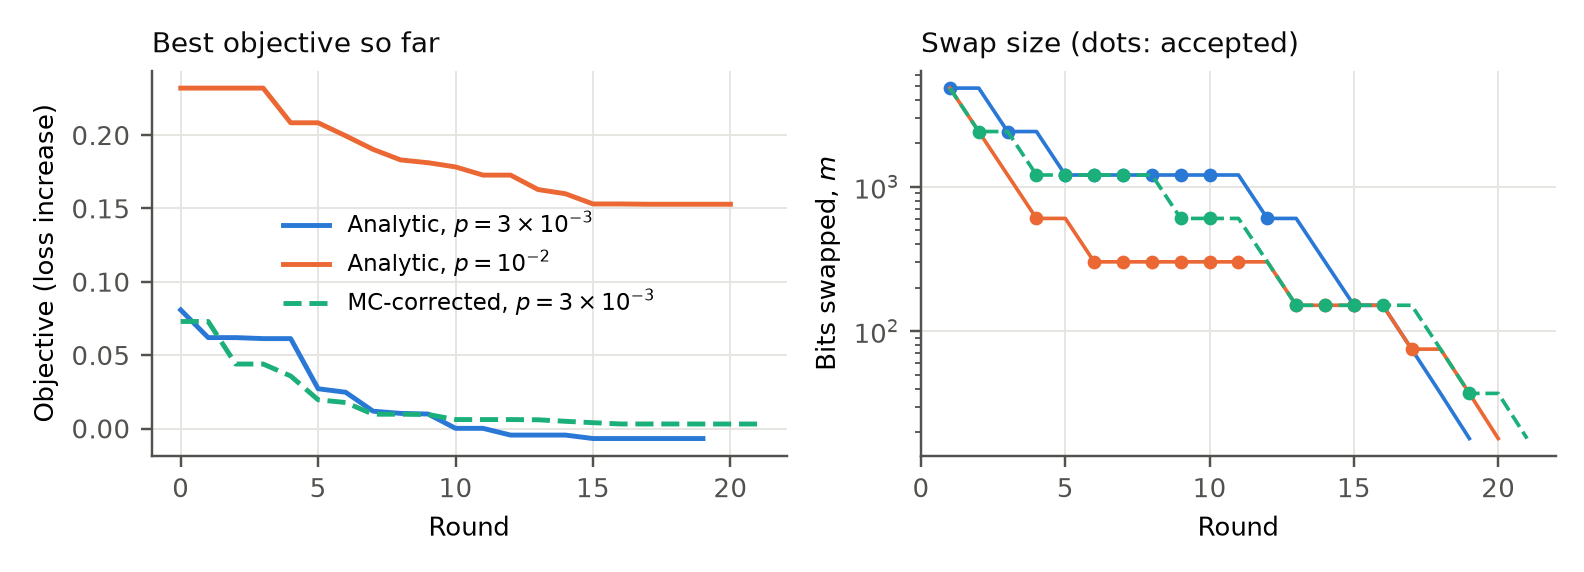
\includegraphics[width=\linewidth]{figures/runr_search_trace.png}
\caption{Course of the rate-aware search, pinned ResNet-8, replication 1, 12.5\% protection, held-out training images. Left: best objective found so far. Right: number of bits swapped per round; dots mark accepted rounds.}\label{fig:trace}
\Description{Objective and swap size per round of the rate-aware search at two bit-error probabilities, analytic and Monte Carlo corrected.}
\end{figure}

\paragraph{Predicted switch rates.} Table~\ref{tab:pstar} gives the frozen predictions of Stage~1 and Fig.~\ref{fig:switch-ckpt} compares them with the measurement for every checkpoint.

\begin{table}[h]
\caption{Predicted switch rate $p^*$ in units of $10^{-3}$, per checkpoint and budget, frozen before the Stage~1 fault fields were drawn. $^\dagger$At the end of the grid ($3\times10^{-2}$).}\label{tab:pstar}
\centering\small
\begin{tabular}{l r r r r r r r r}\toprule
Checkpoint & 1\% & 3.125\% & 6.25\% & 12.5\% & 18.75\% & 25\% & 37.5\% & 50\%\\\midrule
Pinned & 4.9 & 4.1 & 3.7 & 3.5 & 4.0 & 5.2 & 10.5 & 22.0\\
Seed 7101 & 3.3 & 2.8 & 3.3 & 3.1 & 3.6 & 4.9 & 9.0 & 19.4\\
Seed 7102 & 3.7 & 3.7 & 3.5 & 3.4 & 3.8 & 5.1 & 10.6 & 20.8\\
Seed 7103 & 4.1 & 3.5 & 3.3 & 3.2 & 3.9 & 5.2 & 10.6 & 22.0\\
Seed 7104 & 3.4 & 3.2 & 3.3 & 3.2 & 3.6 & 4.8 & 9.7 & 18.4\\
Seed 7105 & 1.6 & 2.6 & 2.4 & 2.6 & 3.2 & 4.5 & 8.8 & 18.4\\
Under-trained & 10.7 & 7.7 & 7.3 & 6.9 & 7.3 & 8.8 & 16.3 & 30.0$^\dagger$\\
Pruned 50\% & 5.4 & 4.9 & 4.8 & 4.8 & 4.9 & 6.0 & 10.5 & 19.2\\
Pruned 70\% & 3.7 & 4.2 & 3.7 & 3.2 & 3.1 & 3.3 & 5.0 & 8.4\\
\bottomrule
\end{tabular}
\Description{Predicted switch rates for nine ResNet-8 checkpoints at eight protection budgets.}
\end{table}

\begin{figure}[h]
\centering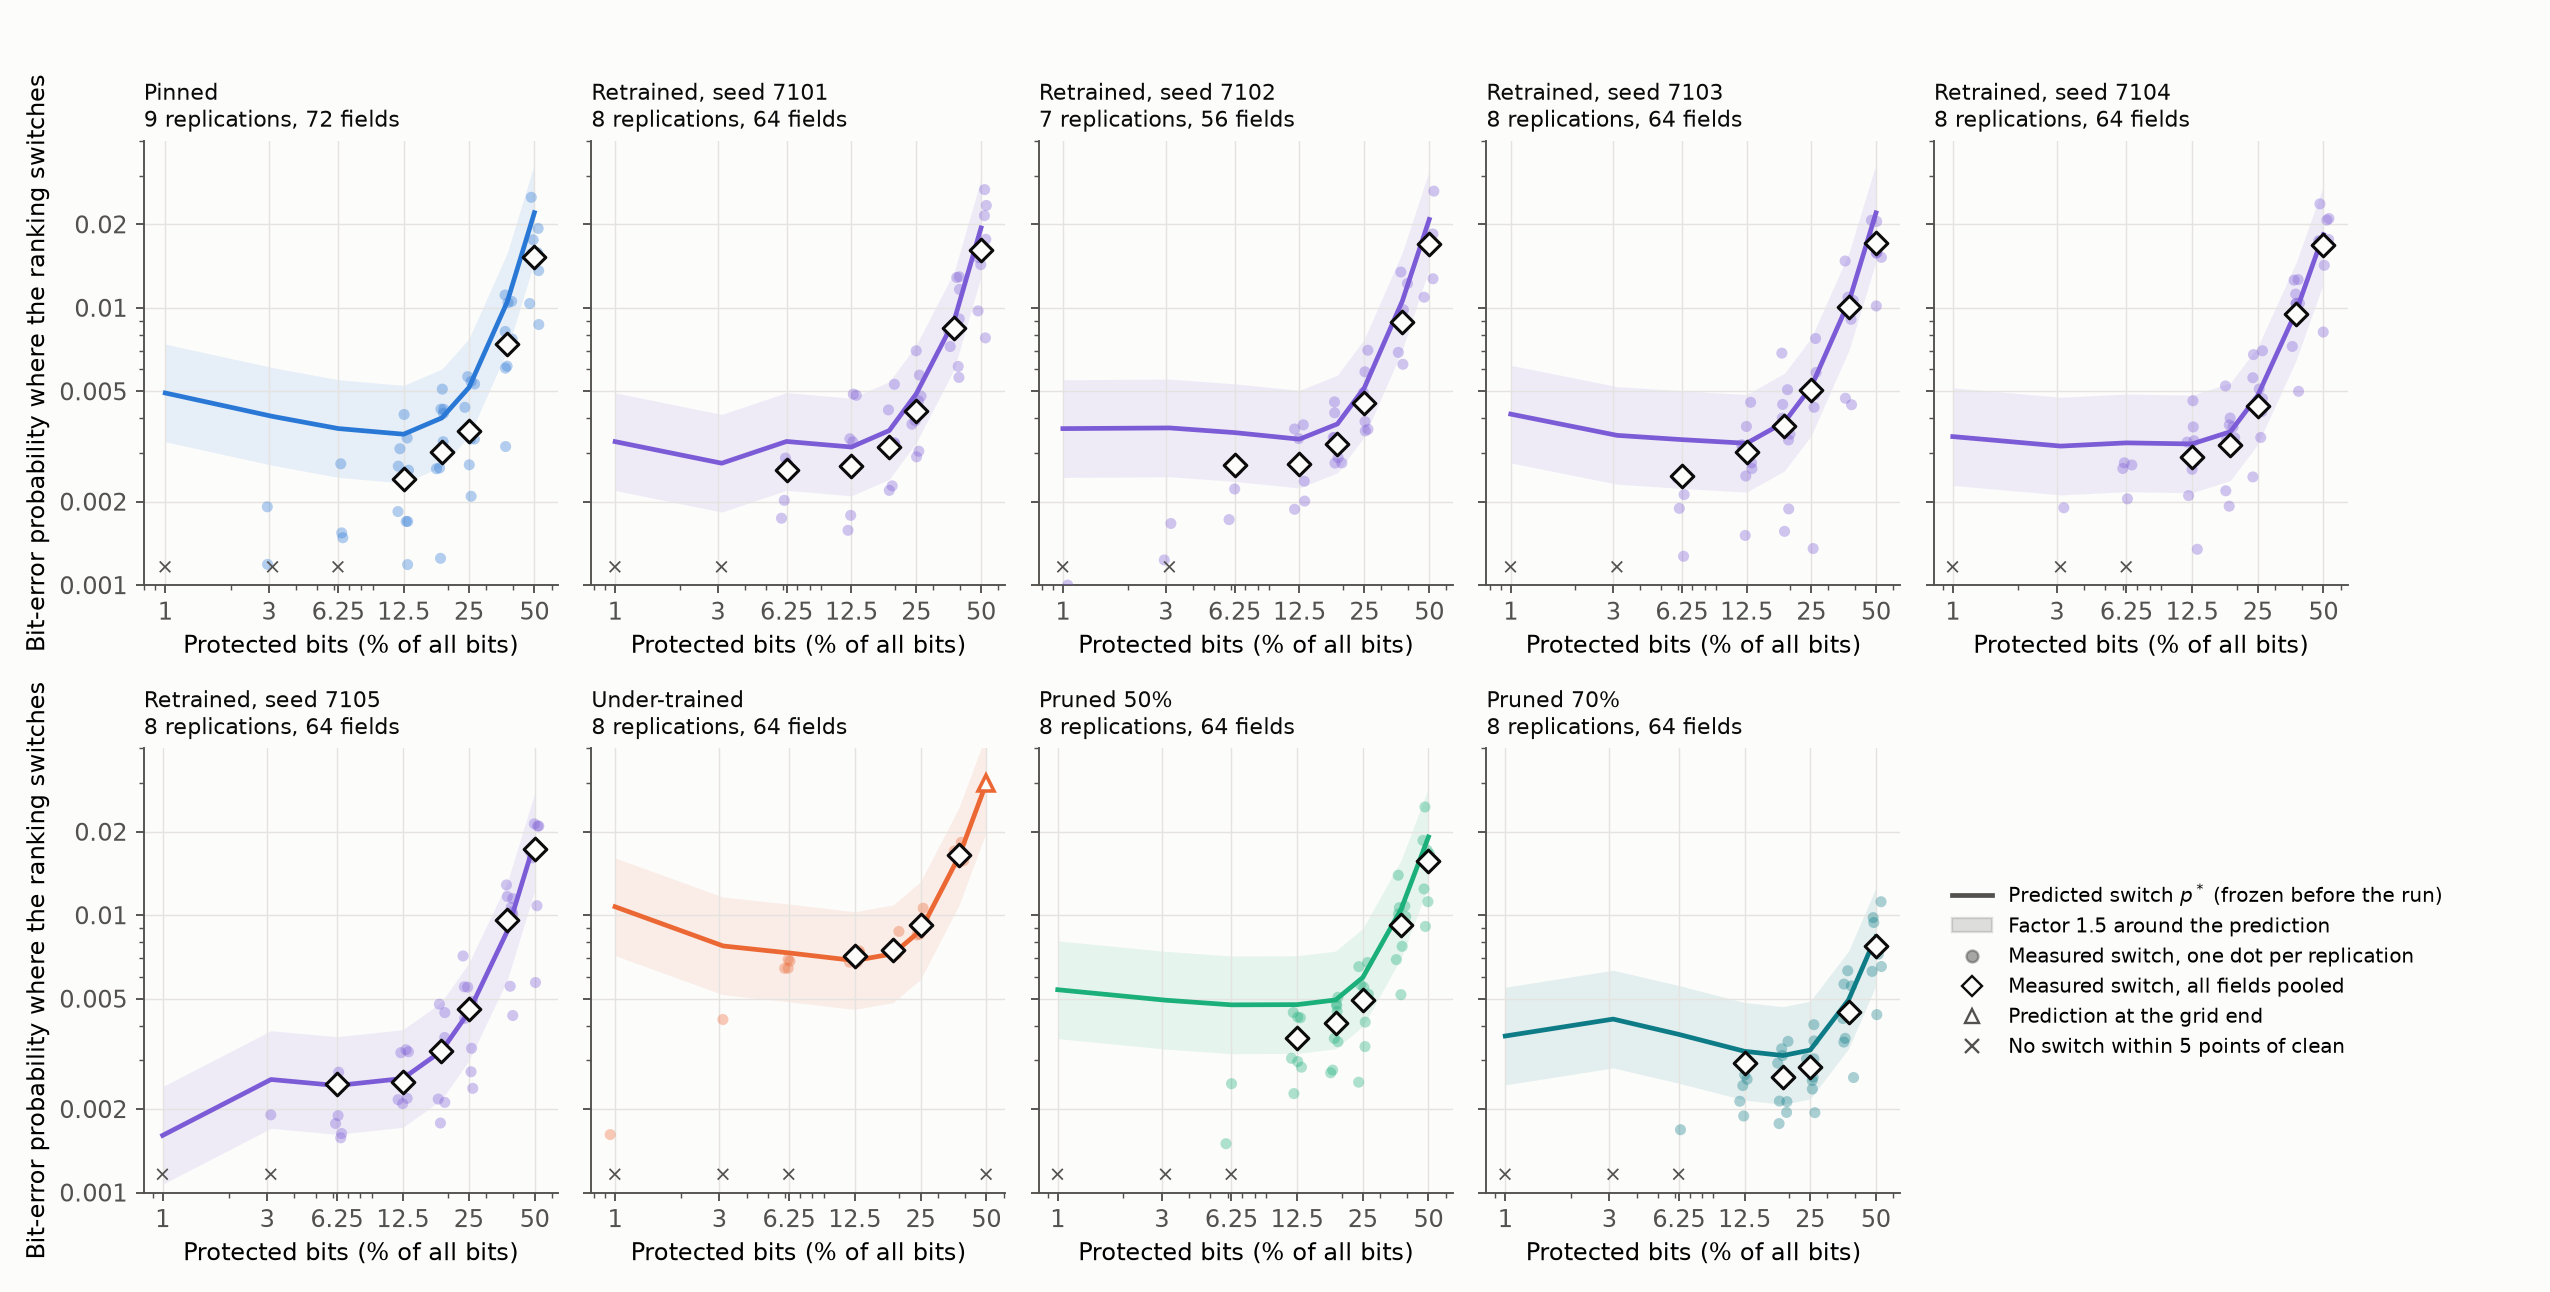
\includegraphics[width=\linewidth]{figures/stage1_switch_per_checkpoint.png}
\caption{Stage 1 per checkpoint: predicted switch (line, with the factor-1.5 band) against the share of protected bits, and the measured switch, per replication (dots) and with all fields pooled (diamonds). Crosses: no switch while the better mask stays within 5 points of clean.}\label{fig:switch-ckpt}
\Description{Nine panels of predicted and measured switch rate against protection budget.}
\end{figure}
